\section{Results discussion}
\subsection{Set Correlation}
The weaker positive relationships between test accuracy and both test kappa and test AUROC in \autoref{fig: test_corr_no_reg} provide insights into the model's performance and its use of the underlying data.

Since the Kappa measure accounts for agreement occurring by chance, a weak correlation with test accuracy might indicate that the dataset's inherent imbalance has not been fully accounted for or that the model performs differently across the classes. It suggests that while accuracy is high, the model might still be biased towards a particular class, i.e., on-task.
AUROC, on the other hand, measures the model's ability to distinguish between classes. A weak correlation with test accuracy could mean that the true positive and false positive rates do not vary proportionately with accuracy.

Thus, a high test accuracy combined with lower test kappa and test AUROC likely means that the model is overfitting the training data and not generalizing well to the unseen data. This implies that the accuracy metric alone is not sufficient to evaluate the model's performance and that the model has not reached its full potential.

In \autoref{fig: reg_type_scatter}, the different regularization techniques are compared in a scatterplot nature, which reveals some clear clusters between the Training and the other sets. Since the y=x line indicates a perfect correlation between the sets, a close fit to this line indicates no overfitting. Hence, even though the L1 metrics score substantially lower on the training set than the other metrics, it's, on average, less overfitted compared to Training and validation. This mainly falls away, though, when considering the test set. L1 mainly worsens the performance on the training set while only slightly improving it on the other sets. The model scoring the highest accuracy on both the Test and validation set used the L1 method; however, this might be more of a case of high variance as there is no clear trend of which method scores the best when comparing the Test and validation set.

The models scoring the highest and closest to the midline on the training validation plot get about an 85\% accuracy on both sets. In contrast, the best models closest to the midline for the validation test sets seem to be in the 65\% area for both sets. Most of these models use the L2 regularization technique.

Comparing the two Test set plots, it's evident that the model overfits the training set, as almost all points score below the midline, signifying higher Training than the test score. The same trend can be seen in the test validation plot, but to a lower degree, indicating that the models are less fitted to the validation set but still overfitted.

In \autoref{fig: reg_val_old}, different regularization values for the L2 method were tested to see which ones scored the best. As expected, higher regularization caused the score on the Training set to decrease, as less overfitting is expected. However...

\subsection{Balance Validation Set}
From the statistics plot \autoref{fig: balance_val}, it's clear that balancing the Validation set outperforms the models not balancing in the extreme, both on the Validation and Test set. This indicated that a balanced Validation set increases the generalization capabilities of the best models. Both parameters scored about the same on the training set, showing higher overfitting for the unbalanced models. 

Comparing \autoref{fig: balance_val_test_auroc} and \autoref{fig: balance_val_val_kappa}, it's clear that the selection metric and selection set greatly impact the model's general performance. Selection by AUROC tends to give a more balanced model with overall high performance. This can be seen in \autoref{fig: memd_data_augmentation_on_test_auroc} through \autoref{fig: memd_data_augmentation_on_val_kappa} as well. The models selected by AUROC also tend to slightly decrease performance from Training to Validation to Test, which is aligned with expectations as the models are expected to be better on seen data and data that performance is selected on. This trend indicated that it's a good selection criterion, that the selected model performs well, and that it is not a random chance. \cite{Jin2019PredictingMW} got an across task accuracy of 60\% which these models score well above. 
\subsection{MEMD Data Augmentation}
From \autoref{fig: memd_data_augmentation_on} through \autoref{fig: memd_data_augmentation_on_val_kappa}, it seems that not adding synthetic data to the dataset leads to the best performances overall. This is quite surprising as IMF-switched synthetic signals are expected to have close to real signal signatures, leading to more data with close to real values. This degradation of the results might be due to the swapping of IMFs or the capture of mind-wandering signatures in the interaction between IMFs, making the synthetic signals more confusing than helpful.
\subsection{MEMD Data Augmentation Ratio}
In \autoref{fig: memd_ratio}, it's clear that the ratios have next to no effect on the performances. This does not fit with the expectation since, from the results of adding synthetic data, we know that this decreases performance. Thus, a natural expectation is that more synthetic data would cause a worse performance, but this is not what is found. 
\subsection{IMF Cleaning}
In \autoref{fig: n_imfs}, all the metrics on the Training set are separated into two distinct groups in the average. The group of 3-5 IMFs and the group with 6,7 and no cleaning. The same trend is observed in accuracy, recall, and F1 on the test set. Looking at \autoref{fig: n_imfs_test_auroc}, the same split is evident, except for a surprisingly bad no-cleaning score. As the no-cleaning models score similarly to the 6 and 7 IMF models in the statistics plot, this might be a case of a particularly bad model scoring very high on the selection criteria and not an indication of more well-selected models. The low IMF models seem less overfitted in the Training set while scoring about the same on the Test set as the models with more IMFs.

\subsection{Early Stopping Patience}
In the statistics \autoref{fig: patience}, the expected result of a positive correlation between higher Patience and higher Training set scores on all metrics. As the Patience goes up, the model gets more overall runs through the training set, leading to overfitting, as can be seen by the average lower scores on the Test set for high patience models. However, as seen in the \autoref{fig: patience_test_kappa} setting, the Patience too low leads to models with too little Training with the medium, 15 to 25, patience models scoring the best on the Test set for the best models. The 20 and 25 patience models score the best for the overall metrics with accuracies of around 78\% and good scores on all other metrics in the Test set, giving higher confidence that the model has learned underlying features. 

\subsection{Regulariazation Techniques}
The statistics plot \autoref{fig: reg_type} is evident from the Training and Test set scores that the L1 is being outperformed. This could be due to too many nodes being effectively set to zero, as explained in \autoref{subsec: regularization}, or it could be that the regularization values tested were too high for the method. To answer this question, a specific L1 regularization value search could be performed in future project iterations.

In \autoref{fig: reg_type_test_auroc}, it's clear that the correlation between the Validation and Test set is highest for the L2 method and that L2 scores substantially higher on Training and Validation than the other methods. It's unsurprising that the L1 scores lower when looking at the statistics plot; however, it's clear from comparing the plots that the no-regularisation case performs well below its max and even average values on the training set. Thus, the model selection methodology of only using AUROC or Kappa on the Test set can lead to bad selections. Still, the L2 method seems to be a solid choice, but further exploration with better model selection is needed.

\subsection{Regularization Values for the L2 method}
As expected, the Training set scores are inversely proportional to the Regularization values, as seen in \autoref{fig: reg_val}. Looking at \autoref{fig: reg_val_test_auroc}, the same trend is evident in the Training set, with the middle values scoring the best on the Test set. In particular, 0.05 and 0.1 give good results for Test Kappa, with good scores on the other test metrics. 

\subsection{Dropout}
As expected, the Training set scores are inversely proportional to the Dropout values, as seen in \autoref{fig: dropout}. On the other hand, the Test set scores are proportional to the Dropout rate on most metrics and had little effect on others in the average case. In the no Droupout case of 0.0 in \autoref{fig: dropout_test_auroc}, a stark difference between Training and Test scores can be seen, indicating strong overfitting, while the 0.8 Dropout rate has a much closer fit between the two sets. Overall, the higher dropout rates seem to have much better correspondence between the different sets, while lower Dropout rates seem more varied. 0.2 seems like an outlier with much better correspondence than 0.0, 0.1, and 0.3, so it might not indicate a good parameter value but instead up to chance.

\section{Generalizability}
As explained in \autoref{sec: results_explanation}, all results were gathered using the General Model with the LOPO validation and test method. Hence, all validation and test set scores reflect model scores on EEG data from unseen participants, meaning the models can generalize well across subjects. This is surprising since EEG data is notoriously subject-specific. Hence, the models must have learned some underlying features shared between subjects. Thus, future expansion of the Transfer model with finetuning on individual subjects might lead to better individual prediction performance. 

The LOPO validation setup might also explain why some models score differently on the test and validation sets. One good way to reduce this discrepancy between the sets would be to opt for an LNPO method using N=2 or N=3 to reduce the variation.

\section{Dataset Critics}
In \autoref{fig: dataset_dist}, duplicated below for convenience, it's clear that the dataset is uneven in the aggregate volume of MW and OT and highly uneven within subjects. This leads to a few takeaways. 

One thing is that the data distribution seems highly unlikely for some subjects. As discussed in \autoref{sec: mind_wandering}, mind wandering is a common phenomenon, and the tasks performed by the subjects under the data collection were likely to induce mind wandering. This makes it unlikely that so many subjects have almost no mind wandering, and thus, many epochs might be mislabeled. Therefore, evaluating epochs as discussed in \autoref{subsec: study_design} could be valuable.

Another aspect is that since EEG signatures are highly individual, the high intra-subject imbalance might worsen any balancing methods. As individual nature worsens, the generalizability between subjects will worsen, and all balancing might need to be done within the subject. If this is the case, it could explain the poor performance of synthetic data found during testing, as all data has only been mixed within the class, not within subjects. However, this would mean that any over- or undersampling would duplicate or delete a lot more data than over- or undersampling in the aggregate, which has been tested. The same is true in the synthetic balancing case, as the synthetic data would be based on much smaller datasets. 
\begin{figure}[H]
    \centering
    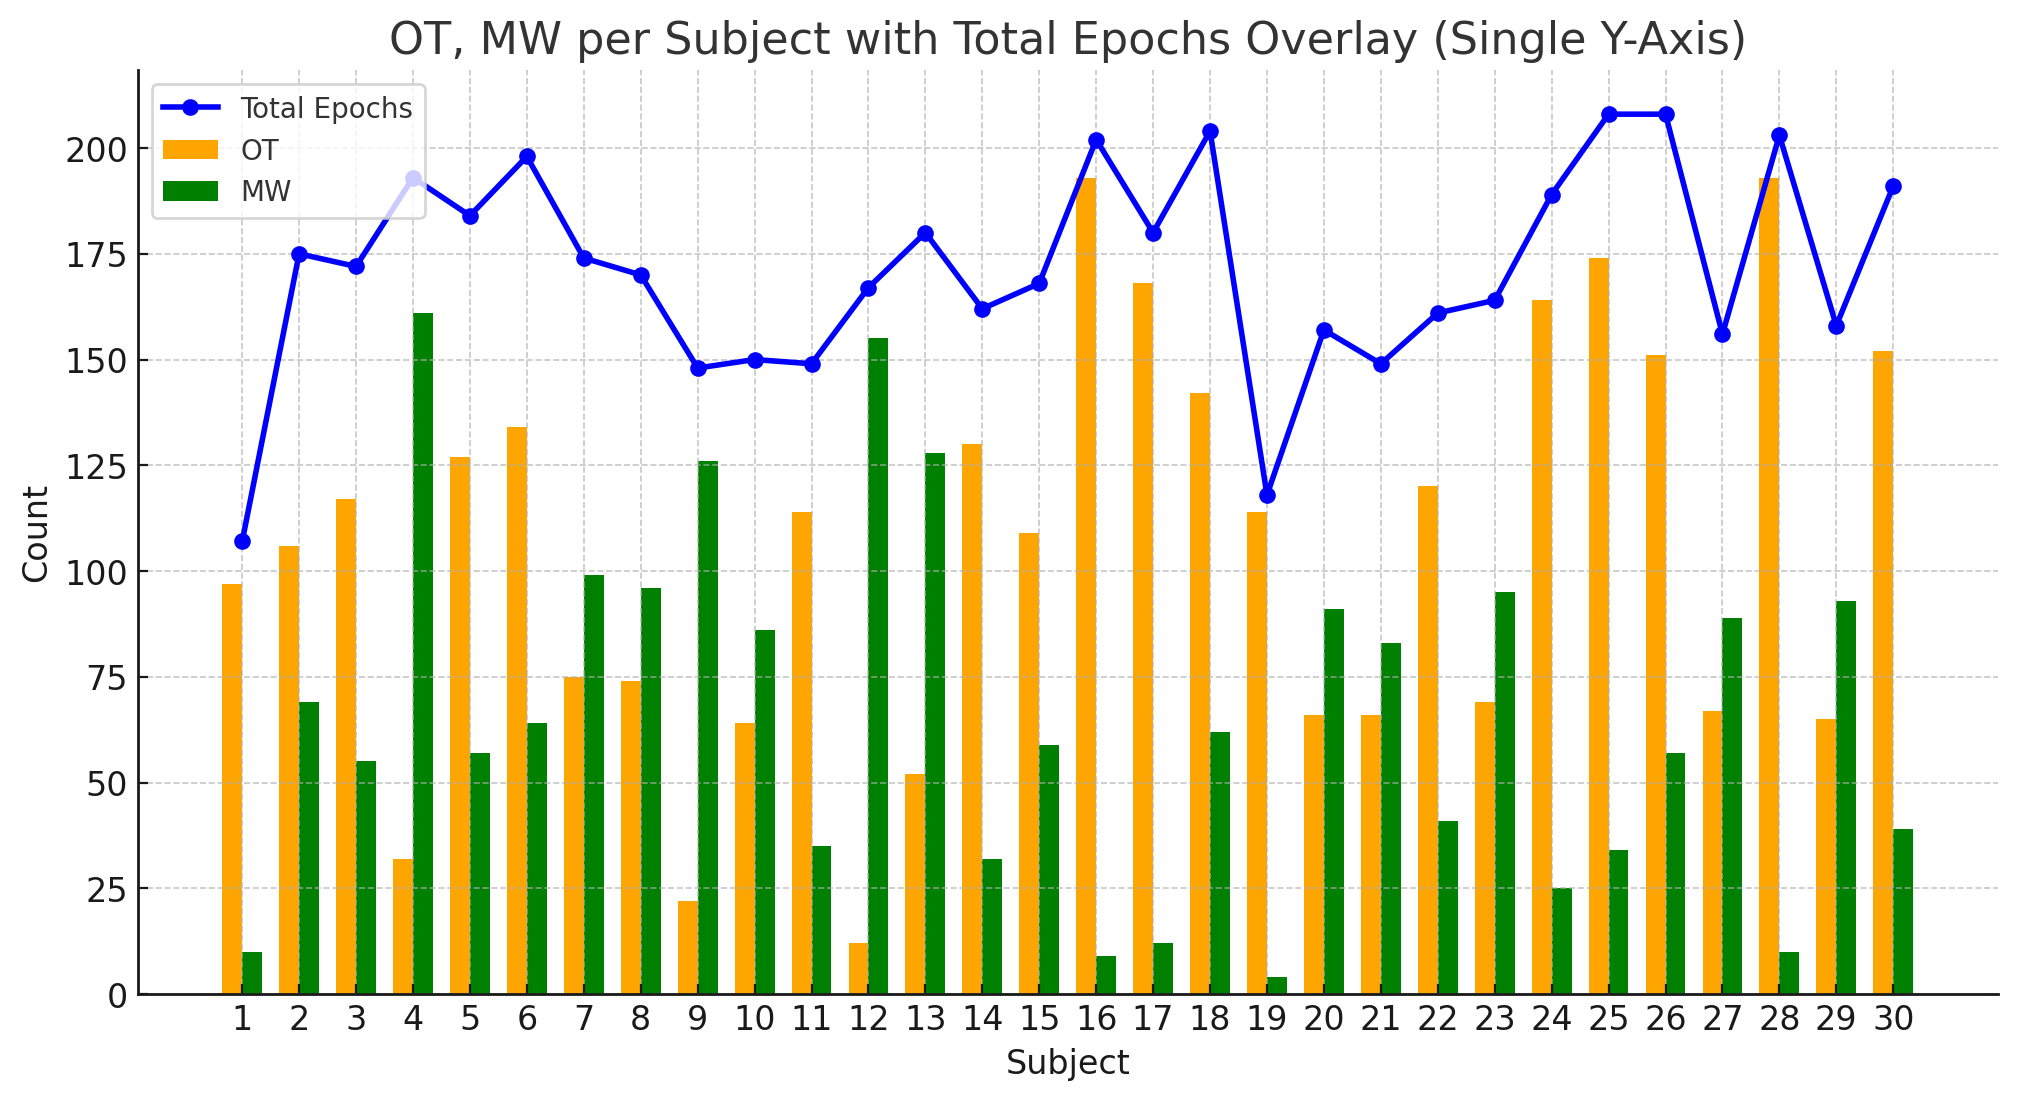
\includegraphics[width=400px]{Figures/dataset_dist.png}
\end{figure}
